
\chapter{Comparison with Experiment}
\label{chapter5}

% 5.1.
\section{ISTTOK}

The ISTTOK project is a reactor based in Lisbon, Portugal, used for plasma science research by the 
University of Lisbon. It is this reactor which found 
no evidence for the existence of anti-parallel currents in the ramp down phase, contradicting 
the hypothesis put forward to explain the presence of a residual plasma during the quiescent 
current cycle, as we discussed in the introduction \cite{malaquias-matthew}. 
This hypothesis was initially supported by data from from the CT-6B tokamak by Huang et. al \cite{huang-ct-tokamak} however, 
and so no consensus exists on whether these currents exist, and what the cause of the runaway electrons is in cases of 
AC tokamak ramp downs. In this chapter we attempt to use our model to describe the current density profile, pressure density profile, 
and poloidal magnetic field topology, given some data provided by ISTTOK.


% 5.1.1
\subsection{Heavy Ion Beam Diagnostics}

The data we have available to us is time slices of current density profile, pressure density profile, 
and $v_{\text{loop}}$ data for the ramp down phase of a run of the ISTTOK reactor. Before 
we ``plug and play'' with this data though, it's important to understand where it has come from. 

One of the flagship features of the ISTTOK reactor is its heavy ion beam probe, which enables 
the measurement of the plasma temperature, electron density, and plasma potential ($v_{\text{loop}}$) 
data. Theoretically it is able to produce a one dimensional profile of each of these components - these 
can then be used to infer the value of other plasma properties, such as the current density profile \cite{ion-beam-diagnostics}.

We will stave off delving too deep into the physics here, and will instead seek to provide an intuition for 
the functioning of the beam. A heavy ion beam is a measurement tool that works by injecting heavy charged 
particles (ions) into a charged medium, at speed. The charged medium in our case is the plasma. For a tokamak, 
a beam of positively charged ions (specifically, atoms with one extra electron) are injected into the plasma, 
known as the ``primary beam'', and commonly consists of one of $\text{Cs}^{+}, \text{Rb}^{+}$. These 
ions are injected perpendicular to the toroidal magnetic field (that is to say, in line with the poloidal 
magnetic field). The idea behind this is that these positively charged atoms ($I^{+}$) will interact with the negatively charged 
electrons in our plasma in a way that we can measure, which will provide us insight into the properties 
of electron populations in our plasma. When $I^{+}$ interacts (collides) with an electron in the plasma, 
it is likely to become ionised further, becoming $I^{2+}$. The property in our plasma that we then 
exploit to measure this change is the Lorentz force, which, to recall, states 
$$\vec{F} = q(\vec{E} + \vec{u} \times \vec{B})$$
where, crucially, $q$ represents a particle's charge as it moves through an magnetic field $B$ with velocity $\vec{u}$, and an electric field $E$ present. 
From this we can infer that the forces acting on a particle will increase as the charge 
increases. The effects of this increased ionisation of our heavy ions thus increases their Larmor radius
(oscillatory movement of charged particles in a magnetic field) relative to their single-ionised counterparts, 
which changes their trajectory in the plasma. In our tokamak we then position a charged particle detector on the opposite 
side of our heavy ion beam's injection point, which we use to measure distributions of received charged 
particles. From this we can infer information about the presence of negatively charged particles 
(predominantly electrons) in the $1D$ profile that our primary beam follows by measuring the 
quantity of charged particles detected at different positions on our detector. Ingenious! A graphic depicting this 
is given in figure \ref{heavy-ion-beam}.

\begin{figure}[h!]
    \centering
    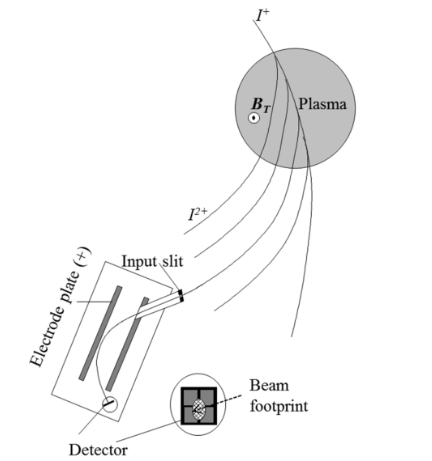
\includegraphics[scale=0.8]{imgs/c5/ion-diagnostics.png}
    \caption{Simplified depiction of an ion beam's injected ions having their trajectories manipulated by the plasma they travel through, and how that is 
    subsequently detected. Diagram taken from \cite{ion-beam-diagnostics}.}
    \label{heavy-ion-beam}
\end{figure}

While here we've provided what is hopefully an intuitive understanding for how a heavy ion beam is utilised for data 
collection in a tokamak, we have skipped much of the nitty-gritty details for actual data derivation. Most importantly for us to note
however, is that ISTTOK does not directly measure the current or pressure density profiles, but instead 
infers this data from poloidal magnetic field profile information afforded to us by the heavy ion beam. 
As one might expect, there is a large margin for 
error introduced in these measurements (and subsequent calculations) when doing so. Quoted unofficially, we can expect errors in 
current density profile data to be up to an order of $\pm30\%$. While we don't have access to the explicit uncertainty in our data, we can keep this in mind when 
fitting our parameters $(a_1, a_2, \alpha)$ to the ISTTOK data, and justify some decisions we make further down.

% 5.1.2
\subsection{Reactor Specification and Data}

\noindent\textbf{Reactor Specification}\\
The ISTTOK reactor specification is given below:

\begin{table}[h!]
    \centering
    \begin{tabular}{|c|c|}
    \hline
    Property           & Value                                                 \\ \hline
    Major Radius ($a$)       & $0.46\text{m}$                                                 \\ \hline
    Minor Radius ($R_0$)      & $0.085\text{m}$                                              \\ \hline
    Plasma Current ($I_p$)   & $~4-6\text{kA}$ \\ \hline
    \end{tabular}
    \caption{Relevant ISTTOK reactor parameters \cite{malaquias-matthew}}
\end{table}

Of particular emphasis, this configuration satisfies the requirement for a large aspect ratio tokamak as required for 
our Grad-Shafranov-Helmholtz model, with $A = R / a = 5.4 \gg 1$ \cite{wang-analytic-solution}. Note that 
aspect ratio in this paper refers to the ratio between major and minor radius, and not the aspect ratio of the cross poloidal 
cross section.

\noindent\textbf{Available Data}\\
\noindent
The data we have is for a series of 20 time slices from $30.53\text{ms} - 31.93\text{ms}$ of 
a run of ISTTOK. Of interest, the average confinement time for a plasma in ISTTOK is approximately
$0.4\text{ms}$ \cite{malaquias-matthew}. For each of these time slices there are $18$ 
measurements at uniformly distributed discrete intervals across the cross section of the reactor; 
for $x \in [-8.5\text{cm}, 8.5\text{cm}]$ and $z = 0$. For this domain we have data for the 
current density profile, and the pressure density profile. From this data, we additionally have inferred $I_p$ and $V_{\text{loop}}$ data for each time slice.

In our simulations we will use the current density profile data to fit our parameters $(a_1, a_2, \alpha)$. 
In the work that we did we did not initially seek to additionally use the pressure density profile data in fitting 
these paramters for two reason:
\begin{enumerate}
    \item We wish to have some data to compare our results to. From the $(a_1, a_2, \alpha)$ we get from our 
    minimisation algorithm we can calculate a pressure density profile and compare it to the experimental data for accuracy
    \item In our simulations we explored the case of having limited current density profile data and attempting to 
    fit parameters to that, and found that we were able to deterine parameters sufficiently accurate to represent the system.
\end{enumerate}
While we will make comparisons with the pressure density profile data, another avenue we could have explored 
was to incorporate the pressure density profile data into our optimisation model (as we discussed potentially doing in chapter \ref{chapter4}). 
We did implement this as a test, however noted that it did not improve the ability of our optimisation algorithm to converge. It is possible 
that, combined with some changes in the approach to fitting our model to data, the inclusion of pressure density profile data could well result in 
a more accurate fit for the model - ideas for future work around this are discussed in chapter \ref{chapter6}.

A representative time slice is provided in figure \ref{current-profile-unnormalised-0}

\begin{figure}[h!]
    \centering
    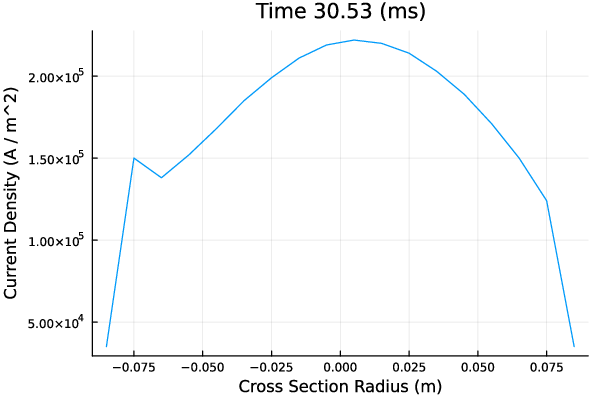
\includegraphics[scale=0.6]{imgs/c5/current-profile-unnormalised-0.png}
    \caption{Current density profile for the beginning of a ramp down in ISTTOK. The cross section radius is centred 
    with respect to the major radius.}
    \label{current-profile-unnormalised-0}
\end{figure}\newpage

The $I_p$ time evolution is also provided for reference in figure \ref{ip-time}. This showcases how the plasma's current 
changes during the ramp down phase.
\begin{figure}[h!]
    \centering
    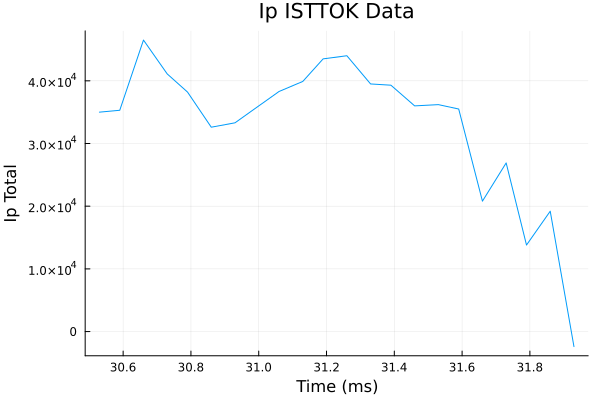
\includegraphics[scale=0.6]{imgs/c5/ip_time_data.png}
    \caption{Plasma current ($I_p$) during the ramp down phase of a run of the ISTTOK reactor in AC operating mode.}
    \label{ip-time}
\end{figure}\newpage

% 5.2
\section{Parameter Fitting}

\subsection{Results}

\subsubsection{Initial Attempts}
We use the same process as we did when initially fitting the parameters $(a_1, a_2, \alpha)$ to data, though instead of contrived 
current inversion data we of course use the data we have from ISTTOK here. Our initial results 
showed a resistance of our model to fitting to the data, as can be seen by the poor fit for 
the current density profile in figure \ref{comparison-current-0-unfiltered}. All of our results are available in the source code under 
under the ``experiments/isttok/current\_solving\_comparison/graphs/'' directory \cite{project-source}.
Here we will highlight a couple representative examples, but will discuss the general trend 
of all our results.

\begin{figure}[h!]
    \centering
    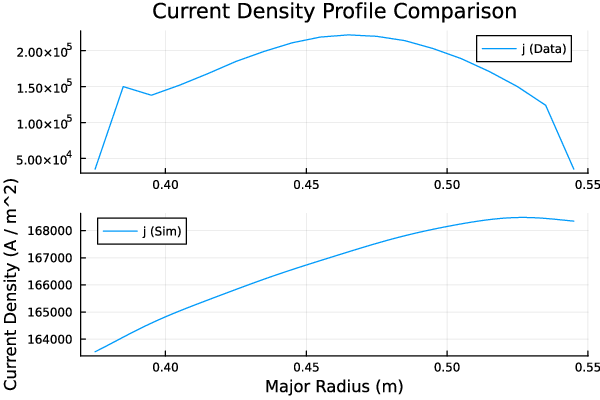
\includegraphics[scale=0.7]{imgs/c5/comparison-current-0-unfiltered.png}
    \caption{ISTTOK current density profile contrasted with our simulated current density profile
    after fitting against the former in order to derive $(a_1, a_2, \alpha)$. This is the first 
    time slice, i.e. at the start of the ramp down.}
    \label{comparison-current-0-unfiltered}
\end{figure}
Purely by visual inspection we can see this is not a close fit, 
however this discrepancy becomes more pronounced as we progress through the remainder of our time slices. 
This effect can be seen in figure \ref{comparison-current-15-unfiltered}, where our simulation is 
even more considerably differentiated from the data.

\begin{figure}[h!]
    \centering
    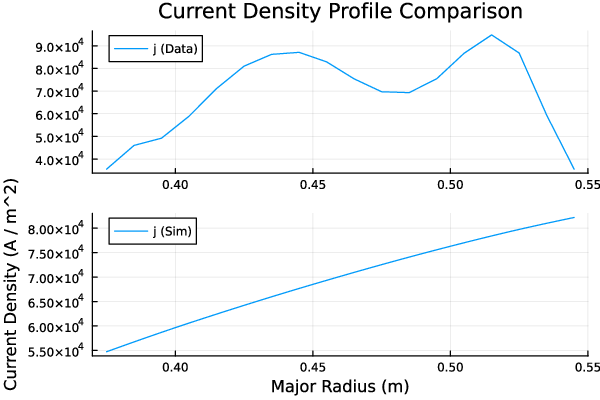
\includegraphics[scale=0.7]{imgs/c5/comparison-current-15-unfiltered.png}
    \caption{ISTTOK current density profile contrasted with our simulated current density profile
    after fitting against the former in order to derive $(a_1, a_2, \alpha)$. This is the 15th 
    time slice, i.e. approximately half way through the transition.}
    \label{comparison-current-15-unfiltered}
\end{figure}

Here we begin to see a current hole develop at (what we for now presume, but will later 
observe) the position of the on-axis magnetic island. This is an important feature to be 
able to characterise in our simulations, however is clearly missed in our simulated current. In fact, 
it seems that the general features of our simulated current density profile remain largely unchanged 
from our initial results - we will comment on why this is so in a minute.

We can also (for completeness here) compare the last time slice, which is the first and only 
data entry we have showing the start of the ramp up phase, or in other words, the period immediately 
proceeding the conclusion of the ramp down phase we are investigating. This comparison is shown 
in figure \ref{comparison-current-20-unfiltered}.
\begin{figure}[h!]
    \centering
    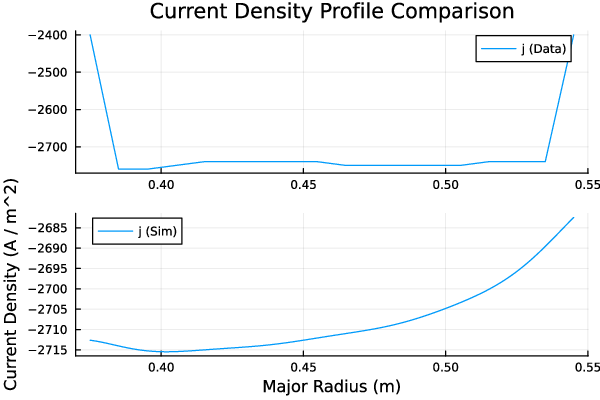
\includegraphics[scale=0.7]{imgs/c5/comparison-current-20-unfiltered.png}
    \caption{ISTTOK current density profile contrasted with our simulated current density profile
    after fitting against the former in order to derive $(a_1, a_2, \alpha)$. This is the last 
    time series data entry we have, and is after the ramp down phase has concluded / the 
    start of the next cycle's ramp up phase.}
    \label{comparison-current-20-unfiltered}
\end{figure}\newpage

Recall that, while the initial parameter guess is currently hand picked (with note on 
alternatives proposed in chapter \ref{chapter6}), parameter guesses for subsequent iterations of our 
simulation are informed by the previously solved-for parameters. This means any initial error in choice of parameters 
will be detrimental to all following simulations.

We can see the effects of this more prominently by also observing the change in magnetic field toplogy 
as the current and pressure data vary. Or rather, we should say, the lack thereof. Figures \ref{mag-field-0} - \ref{mag-field-20}
show the poloidal magnetic field topology for the representative time slices we've picked. Note again that results for all 
time slices can be found in the open sourced GitHub repository \cite{project-source}.

\begin{figure}[h!]
    \centering
    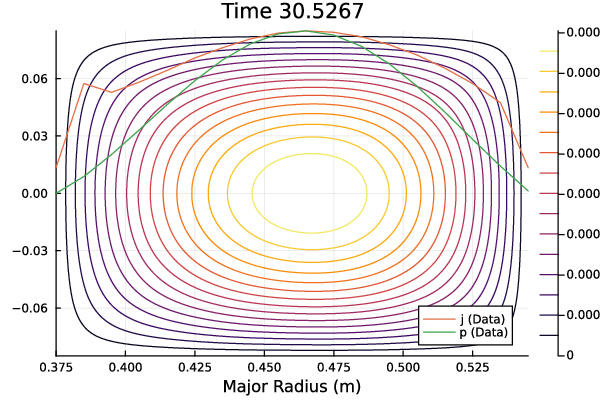
\includegraphics[scale=0.7]{imgs/c5/magnetic-field-0.png}
    \caption{Simulated poloidal magnetic field for a given $(a_1, a_2, \alpha)$ parameter set which is derived 
    from the current density profile data present in the graph. The pressure profile is similarly given. Current and 
    pressure density profiles given are normalised data from ISTTOK.}
    \label{mag-field-0}
\end{figure}\newpage

\begin{figure}[h!]
    \centering
    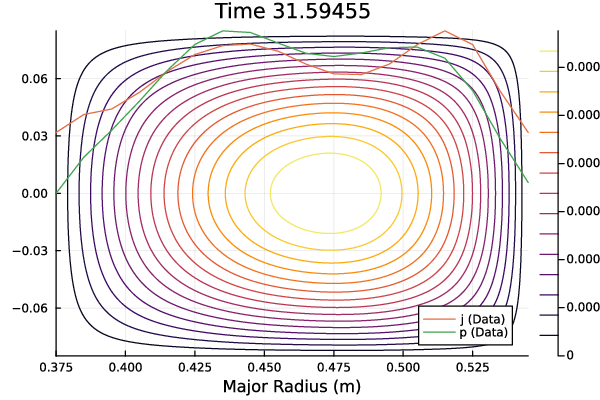
\includegraphics[scale=0.55]{imgs/c5/magnetic-field-15.png}
    \caption{Simulated poloidal magnetic field for a given $(a_1, a_2, \alpha)$ parameter set which is derived 
    from the current density profile data present in the graph. The pressure profile is similarly given. Current and 
    pressure density profiles given are normalised data from ISTTOK.}
    \label{mag-field-15}
\end{figure}

\begin{figure}[h!]
    \centering
    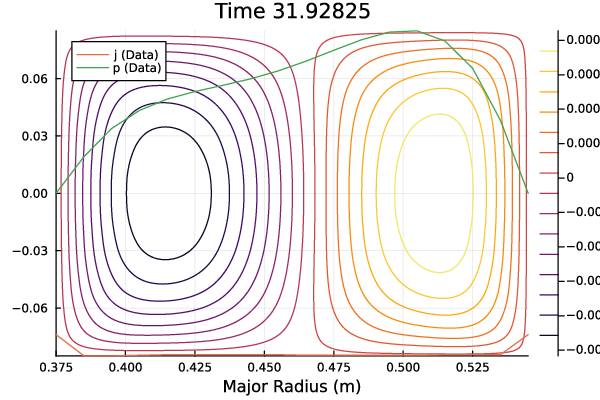
\includegraphics[scale=0.55]{imgs/c5/magnetic-field-20.png}
    \caption{Simulated poloidal magnetic field for a given $(a_1, a_2, \alpha)$ parameter set which is derived 
    from the current density profile data present in the graph. The pressure profile is similarly given. Current and 
    pressure density profiles given are normalised data from ISTTOK.}
    \label{mag-field-20}
\end{figure}\newpage
We find there is minimal variation in magnetic field line toplogy between all the time slices, with exception 
of the last slice, which sees a drastic change. There is a slight drift tendency towards the external wall of the reactor (rightwards in our graphs), 
which might suggest some Shafranov shift of the plasma - though, given the misrepresentative nature of the simulated 
magnetic field lines generally, it is unlikely this is an actual result. We can further support the argument that 
this is not an accurate magnetic field topology as time progresses, as the pressure density profile in 
figure \ref{mag-field-15} suggests the formation of two distinct, or at least a partially split single, plasma, with two 
distinct current densities (i.e., that there are at least two magnetic islands present). However, the simulated magnetic field (which remains largely unchanged from the 
initial simulation iteration) suggests only the existence of a single magnetic island. We should note though, that 
figure \ref{mag-field-0} shows a magnetic field line toplogy which is consistent with where the data suggests the primary 
plasma density should be - this being despite a seemingly large discrepancy between our simulated current density and the 
provided data. Nevertheless, the result is clear - the simulation, in this form, is insufficient in modelling accurately the behaviour of the 
plasma, at least with respect to what is expected from the data we have available.

Our initial efforts seem fleeting in their attempt to accurately model the system. However, that does not mean that 
our efforts should stop there. Whereas previously we politely 
requested any mathematicians avert their gaze at the crimes we were committing, it is only 
fair that we also at some point request any scientists to turn a blind eye to the 
crimes we will momentarily commit. This is that point. 
In the previous section we noted that there is a considerable uncertainty accompanying our data
(see, for instance, figure \ref{ip-time}, which intuitively we expect to be a smooth function of radial distance, 
yet is quite nonsmooth). We thus have some (limited) agency to manipulate our data to be more aligned 
with what we would expect.


\subsubsection{Data Cleanup and Second Attempt}
With the note that our data has considerably uncertainty in it, and considering the 
relatively few data entries we have, we might make some observations about the data 
we do have available, and the general physical properties we would expect it to exhibit 
with relation to the other data points we have available.

First, we will note the (accusedly) extraneous data entries in the first time slice. Refer again 
to figure \ref{current-profile-unnormalised-0}. There are two irregularities we can note:
\begin{itemize}
    \item There is a sharp increase in current density at the $-0.065\text{m}$ offset. Physically, unless 
    there was anomalous behaviour inside the reactor, we would not expect this measurement, while the general 
    behaviour of the rest of the profile relative to this entry is consistent with a plasma density being confined to 
    the magnetic axis within the reactor. Thus, we can (to test) make an assumption that this entry is a result of imprecision in 
    the data collection, and remove it from our fitting data.
    \item At the bounds of the reactor the current density decreases significantly faster than the general trend of the 
    rest of the data. Physically this is consistent with what we would expect - that as we approach the edge of our reactor there is 
    less plasma density and less current. However, we also know our analytic current density profile to be $C^{2}$ continuous, 
    and such sharp jumps will affect our ability to fit to this data. Thus by removing this information we can potentially 
    increase the performance of our data fitting.
\end{itemize}
We see the resulting current density profile in figure \ref{comparison-current-0-edited}. It is clear that the general behaviour 
of our current density profile is more consistent with that of the data now. We can observe that the magnitude of the densities is 
still, however, quite distinct. There are a couple considerations we could make here. First is that, this is evidence that 
our model is not fitting to the data as closely as we'd like yet, and so extra work can be done to attempt to improve this. 
The second would be that, while the scale of the current density is inconsistent with the data, it may be that we can still sufficiently 
make statements about the generation of runaway electron populations, and so it perhaps is (for our intended purposes) irrelevant 
whether the scale is precise or not. More important to us is the topology of the poloidal magnetic field, which in our model is 
informed more by the radial positioning of current density masses than the strength of those densities (as we highlighted in our 
simulations section). We can see in figure \ref{mag-field-edited-data-0} that the magnetic field topology for the manually edited data 
is consistent with where the pressure and current density profiles suggest the primary magnetic island should be. Additionally, it 
appears this is more in agreement than the pre-processed data, as the positioning of the primary magnetic island is more 
accurate to what we expect than we observed in figure \ref{mag-field-0}.

\begin{figure}[h!]
    \centering
    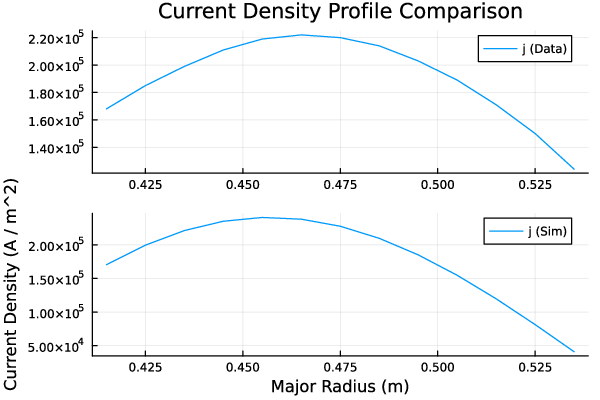
\includegraphics[scale=0.65]{imgs/c5/comparison-current-edited-0.png}
    \caption{Comparison of simulated and data current density profiles, after we rid the data of potentially eroneous data entries.}
    \label{comparison-current-0-edited}
\end{figure}
\begin{figure}[h!]
    \centering
    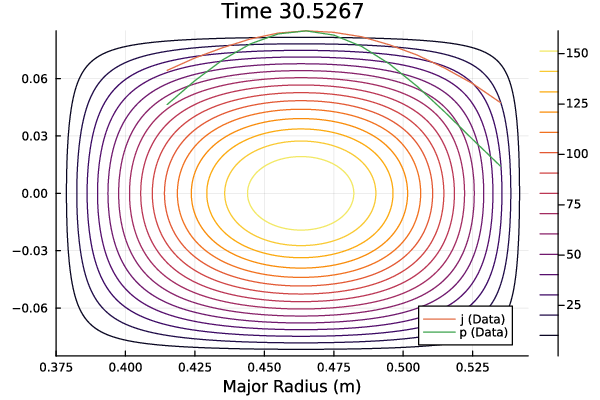
\includegraphics[scale=0.65]{imgs/c5/mag-field-edited-data-0.png}
    \caption{Simulated magnetic field topology for the stripped data. Current and pressure density profiles given are normalised, 
    and provided by the data.}
    \label{mag-field-edited-data-0}
\end{figure}\newpage

These (albeit preliminary) results would seem to suggest that, after some ``cleaning'' of the data, our model is able to 
produce results that are at least consistent with how we would expect our system to behave given the data. 

Nevertheless we face another problem which, as of writing, remains unresolved. While we are able to clean our data 
for the first time slice as what we deemed ``erroneous'' data entries were easy to identify, this is not the case for the majority 
of the remaining data we have. This is partly a problem of labour, more problematic is the that of correctly determining which 
data points to classify as erroneous - if any can even be deemed so.



\subsubsection{Alternative Data Coddling Methods and Steps Forward}
Here we have simply removed potentially erroneous data points from our set, and continued on as if they never existed. 
However, especially as we don't have access to a great many discrete measurements, this is not an ideal situation. 
There are alternative approaches to post-processing the data that could be used, and comparisons made to deem which is 
most suitable for our data fitting purposes. For example, it could be prudent to, after removing these erroneous data points, 
perform an interpolation using the remaining points. This would have the benefit of providing a data set with data that was both 
more volumous, and smoother.

We could also interpolate in another dimension - time. One potential explanation for the difficulty our model has in moving between 
time slices in the data is that the time variation between them is too large with respect to the time perturbation expansion we performed 
in chapter \ref{chapter3}. As such, we could take two consecutive time slices of data and linearly interpolate them, introducing 
many more time slices in between. This would restrict our parameter space further, improving our optimisation, and, combined with 
the previous point about interpolating between data points, could see an improvement on the accuracy of our model.

Additionally, we face the issue that the simulation is very sensitive to the initial parameters chosen. This is directly related 
to the parameter space issue we identified in the chapter \ref{chapter4}, which is that discontinuities introduced by the $\alpha$ 
parameter lead to a high false positive rate. For the above simulations we have achieved some 
results by hand picking an initial parameter guess via manual inspection of the parameter space - this, however, is obviously insufficient 
for more general simulations. A potential resolution for this is proposed in the next chapter, and is the subject of ongoing work.